\section{Umsetzung}
\label{sec:implementation}

Die Umsetzung des Projektes basiert auf einem objektorientierten Ansatz und nutzt Python 2.7.7.

\subsection{Module}
\label{subsec:modules}
Zur Umsetzung der Applikation wurde diese, wie in Abbildung~\ref{fig:module_structure} ersichtlich, in die folgenden Module unterteilt:

\begin{compactitem}
\item \textit{algorithms}\\
    Enthält Algorithmen zur Lösungsfindung
\item \textit{controller}\\
    Enthält die komplette Steuerung des Spiels, sowie die grundlegenden Elemente
\item \textit{player}\\
    Enthält Spieler zur Durchführung des Spiels
\end{compactitem}

\begin{minipage}[]{1.0\textwidth}

    \centering
    \begin{minipage}[t]{0.5\textwidth}
        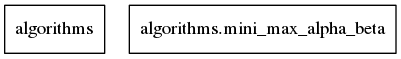
\includegraphics[width=\textwidth]{images/packages_algorithms.png}
    \end{minipage}
    \begin{minipage}[t]{0.3\textwidth}
        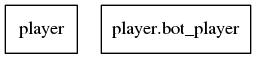
\includegraphics[width=\textwidth]{images/packages_player.png}
    \end{minipage}
    \begin{minipage}[t]{0.95\textwidth}
        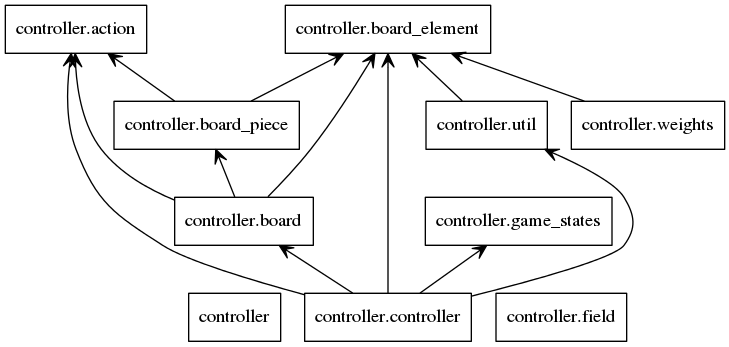
\includegraphics[width=\textwidth]{images/packages_controller.png}
    \end{minipage}

\captionof{figure}{Modulstruktur der Applikation\protect\footnotemark}
\label{fig:module_structure}
\end{minipage}
\footnotetext{Eigene Darstellung mittels Pyreverse (http://www.logilab.org/blogentry/6883)}

\newpage

\subsection{Klassenstruktur}
\label{subsec:class_structure}
Die Applikation besteht aus den in der Abbildung~\ref{fig:class_structure} abgebildeten Klassen und Attributen.

\begin{minipage}[]{1.0\textwidth}

    \centering
    \begin{minipage}[t]{0.2\textwidth}
        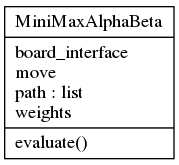
\includegraphics[width=\textwidth]{images/classes_algorithms.png}
    \end{minipage}
    \begin{minipage}[t]{0.22\textwidth}
        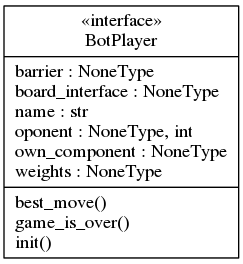
\includegraphics[width=\textwidth]{images/classes_player.png}
    \end{minipage}
    \begin{minipage}[t]{0.7\textwidth}
        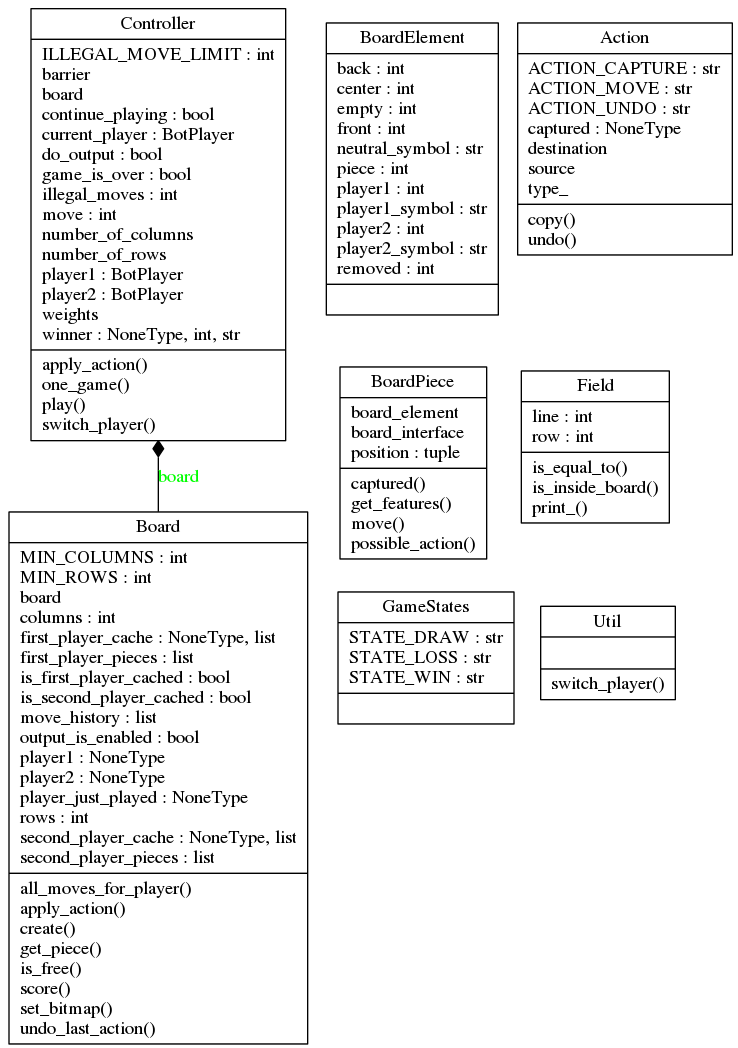
\includegraphics[width=\textwidth]{images/classes_controller.png}
    \end{minipage}

\captionof{figure}{Klassendiagramm der Applikation\protect\footnotemark}
\label{fig:class_structure}
\end{minipage}
\footnotetext{Eigene Darstellung mittels Pyreverse (http://www.logilab.org/blogentry/6883)}

\subsection{Programmablauf}
\label{subsec:program_flow}

Grundsätzlich ist die Applikation so aufgebaut, dass sie direkt mittels dem Controller-Interface initialisiert und dann gestartet werden kann. Die Berechnung bzw.\ der Ablauf des Spiels läuft dann vollkommen automatisch ab. Schlussendlich wird eine Meldung über den Gewinner bzw.\ ob ein Unentschieden erreicht wurde ausgegeben.

Der hauptsächliche Teil des Programmablaufs findet --- wie der Name bereits andeutet --- im \textit{Controller}-Modul statt. Dieses startet eine Schleife, welche so lange läuft, wie das Spiel nicht beendet ist. Zusätzlich wurde eine Limit eingebaut, welche nach Erreichen das Spiel mit einem Unentschieden abbricht. Dies wurde so gewählt, da es möglich ist, dass keine Relevanten Züge mehr geschehen und es so unter Umständen --- bei einer sehr passiven Strategie der Spieler --- zu keinem Ende kommt.

Innerhalb der Schleife wird quasi Zug nach Zug pro Spieler berechnet, wobei pro Zug die Seite gewechselt wird. Für jeden Spieler wird pro Zug vom Controller aus der beste Zug abgefragt. Der Spieler evaluiert dies, indem er alle möglichen Züge durch das Interface des Spielbretts abfragt und dann mittels einem gewählten Algorithmus eine Evaluation --- bis zu einer gewissen Tiefe --- durchführt. Die Schnittstelle des Spielers ist generisch gehalten, so dass ein Spieler im Prinzip einen beliebigen Algorithmus zur Evaluation des besten Zuges anwenden kann. Aktuell wurde jedoch nur der MiniMax-Algorithmus mit Alpha-Beta-Pruning umgesetzt.

Hat der Spieler einen von ihm aus gesehen besten Zug evaluiert, meldet er dies dem Controller, welcher dann den Zug durch das Interface des Spielbretts auf dieses anwendet. Als Abbruchkriterium dient hier ob ein Spieler entweder keine Steine mehr zur Verfügung hat oder aber ein Spieler keine erlaubten Züge (Bewegung auf ein freies Feld, Überspringung des Gegners) vornehmen kann.

In den Abbildungen~\ref{fig:program_flow_01} und~\ref{fig:program_flow_02} wird das gerade Genannte visuell verdeutlicht.

\newpage

\begin{minipage}[]{1.0\textwidth}

    \centering
    \begin{minipage}[t]{0.7\textwidth}
        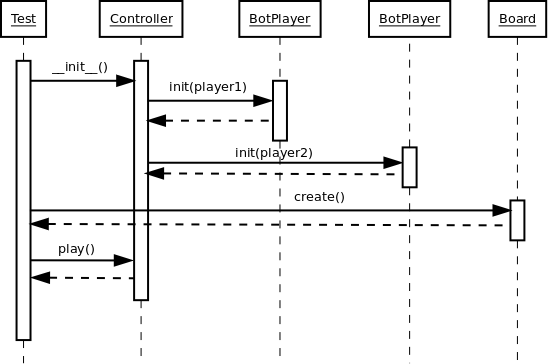
\includegraphics[width=\textwidth]{images/program_flow_01.png}
        \captionof{figure}{Initialisation der Applikation\protect\footnotemark}
\label{fig:program_flow_01}
    \end{minipage}

    \hspace{1cm}

    \begin{minipage}[t]{0.8\textwidth}
\label{fig:program_flow_02}
        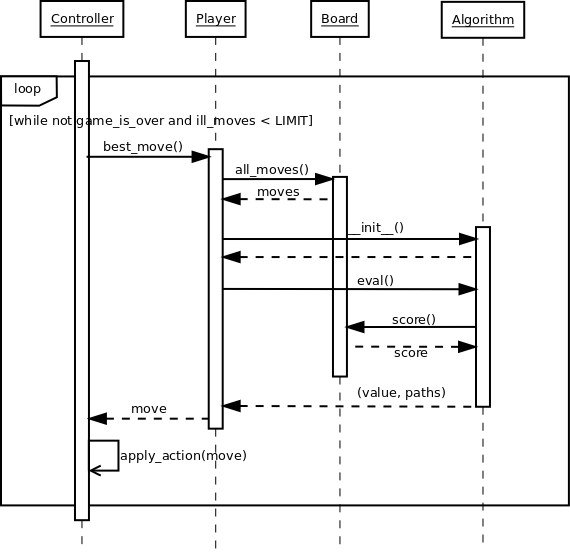
\includegraphics[width=\textwidth]{images/program_flow_02.png}
        \captionof{figure}{Eigentlicher Ablauf der Applikation\protect\footnotemark}
\label{fig:program_flow_02}
    \end{minipage}
\end{minipage}
\addtocounter{footnote}{-2} %3=n
 \stepcounter{footnote}\footnotetext{Eigene Darstellung mittels Dia}
 \stepcounter{footnote}\footnotetext{Eigene Darstellung mittels Dia}
